\section{Systems of Differential Equations}
When studying physical systems, higher order differential equations often arise, therefore a procedure to work on these models has to be presented. Another important reason to present the following methodology is that the numerical algorithms presented require the form of equation \eqref{eq:iode}, i.e. individual first order differential equations.

\subsection{Phase Variables}
The following procedure was obtained from \cite{rowell2002state} and \cite{antsaklis2006linear}. Suppose you have a system described by
\begin{equation}\label{eq:generalDiff}
\begin{cases}
    y^{(n)}(t)=f\left(y^{(n-1)},...,y'',y',y,t\right) &\\ y(0)=y_0,\,\dots,\,y^{(n - 1)}(0)= y_{(n - 1)}\quad t\in[0,T]&
\end{cases}
\end{equation}

and a solution is desired in an interval $[0,T]$. In order to convert this system into a system of first order differential equations, let us make the substitution in the phase variables, which allow us to represent the original system \eqref{eq:generalDiff} as follows
\begin{equation}
    \begin{cases}
        x_1 = y&\\
        x_2 = y'&\\
        \qquad\vdots&\\
        x_n = y^{(n-1)}&
    \end{cases}\longrightarrow
     \begin{cases}
        x'_1=x_2&\\
        x'_2=x_3&\\
        \qquad\vdots&\\
        x'_{n-1}=x_n&\\
        x'_n=f\left(x_n,x_{n-1},...,x_2,x_1,t\right)
    \end{cases}
\end{equation}
\begin{equation*}
    x_1(0)=y_0,\dots,\,x_{n - 1}(0)= y_{(n - 1)}
\end{equation*}

This system can be synthesized as 
\begin{equation}\label{eq:syn_sys_odes}
\begin{cases}
    \mathbf{x}'=F(\mathbf{x},t) &\\ \mathbf{x}(0) = \mathbf{x}_0\quad t\in[0,T]&
\end{cases}
\end{equation}
where $\mathbf{x}=[x_1\,\,x_2\,\,...\,\,x_n]^T$ is the state vector. Now we have obtained a set of $n$ first-order ordinary differential equations. In the following section, we will present how to work on these systems using the already presented methods.

\subsection{Numeric Simulation}
    \subsubsection{Euler}
    If it is wanted to simulate a system of first order differential equations through Euler's method, the following procedure is based on the original from section \ref{sec:euler} but with a slight twist: vectors instead of scalars.

    Let \[\mathbf{x}(j)=\left[x_1(j)\,\,x_2(j)\,\,\dots\,\, x_n(j)\right]^T\]
    be values of the $n$ variables of the system of $n$ differential equations at the iteration $j$. The iterative process to obtain the approximated solution is
    \begin{equation}
        \mathbf{x}(j+1)= \mathbf{x}(j)+hf(t_j,\mathbf{x})
    \end{equation}
    
    
    \subsubsection{Fourth-order Runge-Kutta}
    In order to simulate a system of differential equations with RK4, we use the same procedure described in section \ref{sec:rk4}, but treating the variable as a vector of variables. For a system of $n$, the recurrence formula for RK4 method will be
    \begin{equation}
        \mathbf{x}\left(j+1\right) = \mathbf{x}(j) + \dfrac{h}{6}\left(\mathbf{k}_1 + 2\mathbf{k}_2 + 2\mathbf{k}_3 + \mathbf{k}_4\right)
    \end{equation}
    Where: \[\mathbf{x}(j)=\left[x_1(j)\,\,x_2(j)\,\,\dots\,\, x_n(j)\right]^T\,\,\mathbf{k}_i=\left[k_{ix_1}\,\, k_{ix_2}\,\,\dots\,\, k_{ix_n}\right]^T\quad i=1,\,\dots,\,4\]
    And $k_{1x_k}$, $k_{2x_k}$, $k_{3x_k}$ and $k_{4x_k}$ will be defined exactly as they have been already shown in section \ref{sec:rk4}, but for each variable $x_k$. It is important to note that the simulation has to be performed sequentially, that is, it is necessary to calculate the whole state vector $\mathbf{x}$ at a time $t$ in order to calculate the next state vector at a time $t+1$.

    
    \begin{exmp} Higher Order ODEs: Consider the Duffing oscillator
    \begin{equation}
        y''+\delta y'+\alpha y+\beta y^{3}=\gamma \cos (\omega t)
    \end{equation}
    which has a wide variety of real applications in physical systems (see \cite{Korsch2008}). The equivalent system of first order ODEs is
    
    
    \begin{equation}
        \begin{cases}
        x_1 = y&\\
        x_2 = y'&\\
    \end{cases}\longrightarrow
    \begin{cases}
        x_1'=x_2&\\
        x_2'=-\delta x_2-\alpha x_1-\beta x_1^3 + \gamma\cos(\omega t)
    \end{cases}
    \end{equation}
    \end{exmp}
    
    Now we have a system of first order ODEs just as \ref{eq:syn_sys_odes}; now, Euler's or RK4 methods can be applied. The following simulation was performed using RK4 for $T=200s$ with $h=0.01$ with parameters $\delta=0.3$, $\alpha =-1$, $\beta=1$,$\gamma=0.37$, $\omega =1.2$ and initial conditions $x_1(0)=1$,  $x_2(0)=0$. The results are presented in figure \ref{fig:duffing}.
    
    \begin{figure}[H]
    \centering
    \begin{subfigure}[ht]{0.45\textwidth}
    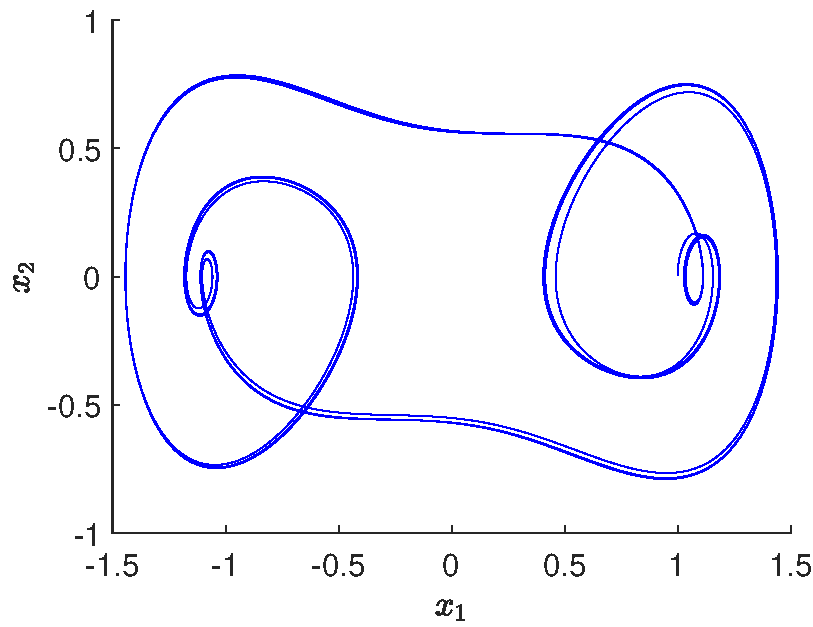
\includegraphics[scale=0.38]{files/duffing_phase.pdf}
    \end{subfigure}
    \begin{subfigure}[ht]{0.45\textwidth}
    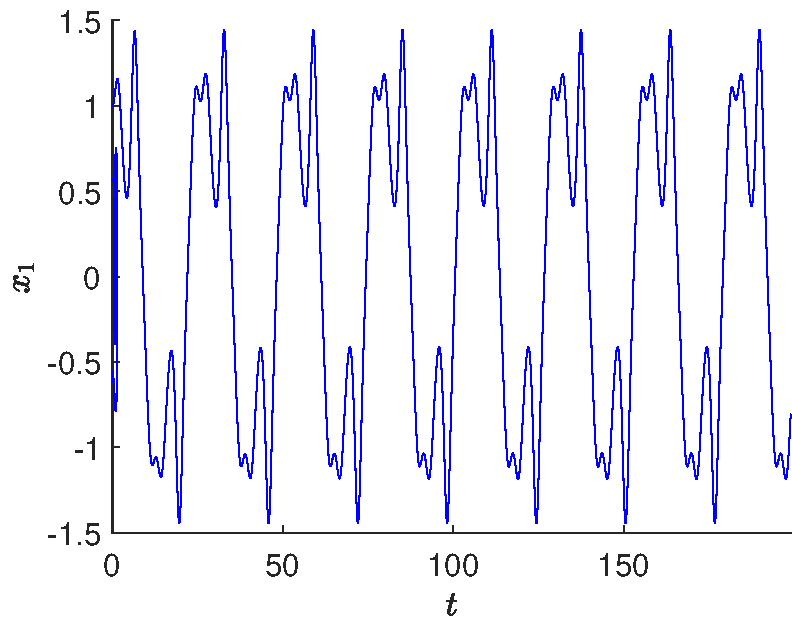
\includegraphics[scale=0.38]{files/duffing_time.pdf}
    \end{subfigure}
    \caption{Duffing oscillator simulation.}
    \label{fig:duffing}
    \end{figure}
    
    Although presented algorithms can be applied directly to systems of ODEs, let us show an example using RK4:
\begin{exmp} System of First Order ODEs:
    The Lotka-Volterra equations (predator-prey model) is a system of ODEs as follows:
\begin{equation}
    \begin{cases}{y_1'=\alpha y_1-\beta y_1 y_2}& \\ {y_2'=\delta y_1 y_2-\gamma y_2}&\end{cases}
\end{equation}
where $y_1$ represents the number of preys and $y_2$ is the amount of predators.

\begin{figure}[H]
    \centering
    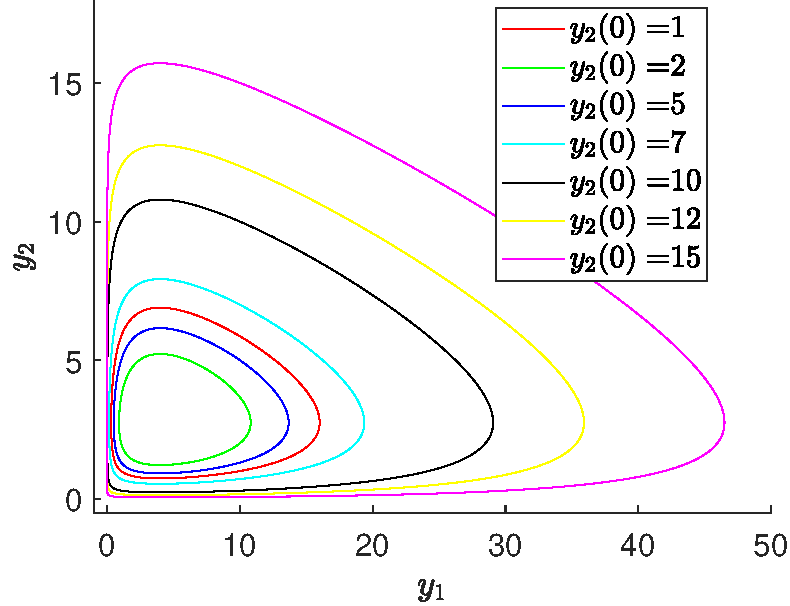
\includegraphics[scale=0.4]{files/Prey.pdf}
    \caption{Phase portrait of Lotka-Volterra equations.}
    \label{fig:lotka}
\end{figure}
\end{exmp}
